\documentclass[format=acmsmall, review=false]{acmart}
\usepackage{acm-ec-26}
\usepackage{booktabs}
\usepackage{graphicx}
\setcitestyle{authoryear}
% Generated by python -m research.facts. Do not edit.
\newcommand{\activeGap}{7}
\newcommand{\activeZone}{14\%}
\newcommand{\backedFifteen}{+7.2\% (-0.3 to +14.3)}
\newcommand{\backedFive}{+8.7\% (-0.6 to +17.6)}
\newcommand{\backedMarkets}{2,415}
\newcommand{\backedOne}{+18.6\% (+4.7 to +34.0)}
\newcommand{\backedSixty}{+0.8\% (-6.9 to +7.6)}
\newcommand{\backedStakeM}{7.0}
\newcommand{\brierOverall}{0.107}
\newcommand{\dBrierBlendAll}{-0.00220 (-0.00260 to -0.00179)}
\newcommand{\dBrierBlendHold}{-0.00183 (-0.00254 to -0.00115)}
\newcommand{\dBrierIsotonicAll}{+0.00014 (+0.00003 to +0.00026)}
\newcommand{\dBrierIsotonicHold}{+0.00036 (+0.00016 to +0.00055)}
\newcommand{\dBrierMidAll}{-0.00022 (-0.00084 to +0.00039)}
\newcommand{\dBrierMidHold}{-0.00213 (-0.00317 to -0.00112)}
\newcommand{\dBrierPlattAll}{+0.00012 (-0.00002 to +0.00025)}
\newcommand{\dBrierPlattHold}{+0.00051 (+0.00026 to +0.00074)}
\newcommand{\dBrierResFlowAll}{-0.00094 (-0.00123 to -0.00063)}
\newcommand{\dBrierResFlowHold}{-0.00134 (-0.00175 to -0.00093)}
\newcommand{\dBrierResFullAll}{-0.00210 (-0.00248 to -0.00170)}
\newcommand{\dBrierResFullHold}{-0.00273 (-0.00337 to -0.00210)}
\newcommand{\displayedRule}{+53\% (+50 to +56)}
\newcommand{\dormantGap}{14}
\newcommand{\dormantShare}{32\%}
\newcommand{\dormantZone}{38\%}
\newcommand{\encModel}{0.60 (0.39 to 0.69)}
\newcommand{\encPrice}{0.52}
\newcommand{\encUpdown}{0.07 (-0.03 to 0.20)}
\newcommand{\fadeFillUsd}{5}
\newcommand{\fadeHigh}{+23.4\% (+15.4 to +31.9)}
\newcommand{\fadeHighBase}{+38.3\% (+31.7 to +45.5)}
\newcommand{\fadeHighLate}{+31.8\% (+20.7 to +43.7)}
\newcommand{\fadeHighN}{4,598}
\newcommand{\fadeMid}{+15.5\% (+10.8 to +20.0)}
\newcommand{\fadeMidBase}{+17.5\% (+14.1 to +20.9)}
\newcommand{\fadeMidLate}{+16.7\% (+10.7 to +22.8)}
\newcommand{\fadeMidN}{5,282}
\newcommand{\fadeTotalK}{176}
\newcommand{\fadeWait}{73}
\newcommand{\firstEntryHigh}{-3.80\% (-4.18 to -3.40)}
\newcommand{\firstEntryHighN}{37,857}
\newcommand{\firstEntryMid}{-2.65\% (-3.25 to -2.03)}
\newcommand{\firstEntryMidN}{31,956}
\newcommand{\firstTimers}{-1.14\% (-2.07 to -0.05)}
\newcommand{\ftHigh}{-11.3 (-12.4 to -10.1)}
\newcommand{\ftHighMag}{11.3 (10.1 to 12.4)}
\newcommand{\ftLow}{+3.1 (+2.7 to +3.6)}
\newcommand{\ftMarkets}{21,003}
\newcommand{\ivRatioHigh}{0.99}
\newcommand{\ivRatioLow}{0.97}
\newcommand{\lastQuarter}{2026Q3}
\newcommand{\lastQuarterEndorsed}{+2.6\% (-17.9 to +18.8)}
\newcommand{\llmBase}{0.243}
\newcommand{\llmBlindFable}{0.236}
\newcommand{\llmBlindHaiku}{0.246}
\newcommand{\llmBlindSonnet}{0.235}
\newcommand{\llmMarket}{0.153}
\newcommand{\llmN}{282}
\newcommand{\llmPriceFable}{0.154}
\newcommand{\llmPriceHaiku}{0.152}
\newcommand{\llmPriceSonnet}{0.155}
\newcommand{\modelMarketBrier}{0.1124}
\newcommand{\modelTestMarkets}{36,398}
\newcommand{\nMarkets}{1,009,373}
\newcommand{\opposedFifteen}{-3.9\% (-8.4 to +0.5)}
\newcommand{\opposedFive}{-4.8\% (-10.1 to +0.8)}
\newcommand{\opposedOne}{-10.2\% (-18.2 to -1.9)}
\newcommand{\opposedOneLoss}{10.2\% (1.9 to 18.2)}
\newcommand{\opposedSixty}{+0.5\% (-3.8 to +4.9)}
\newcommand{\plHoldBlend}{+9.2\%}
\newcommand{\plMarkets}{13,357}
\newcommand{\plMidBlend}{+11.5\%}
\newcommand{\plMidBlendCI}{-0.00862 (-0.00955 to -0.00770)}
\newcommand{\plMidFair}{+10.9\%}
\newcommand{\plSkillBlend}{+8.3\%}
\newcommand{\plSkillFair}{+7.6\%}
\newcommand{\pooledHigh}{+6.5 (+3.9 to +8.6)}
\newcommand{\pooledHighMag}{6.5 (3.9 to 8.6)}
\newcommand{\quoteMarketsK}{170}
\newcommand{\replayAll}{+8.1\%}
\newcommand{\replayCapitalK}{379}
\newcommand{\replayConfirm}{+1.5\%}
\newcommand{\replayConfirmT}{0.33}
\newcommand{\replayDSR}{0.38}
\newcommand{\replayPnlK}{624}
\newcommand{\replaySharpe}{1.33}
\newcommand{\replayT}{1.76}
\newcommand{\seasoned}{+0.55\% (+0.17 to +0.98)}
\newcommand{\skillBlendAll}{+1.96\%}
\newcommand{\skillBlendHold}{+1.47\%}
\newcommand{\skillIsotonicAll}{-0.13\%}
\newcommand{\skillIsotonicHold}{-0.29\%}
\newcommand{\skillMidAll}{+0.20\%}
\newcommand{\skillMidHold}{+1.71\%}
\newcommand{\skillPlattAll}{-0.11\%}
\newcommand{\skillPlattHold}{-0.41\%}
\newcommand{\skillResFlowAll}{+0.84\%}
\newcommand{\skillResFlowHold}{+1.08\%}
\newcommand{\skillResFullAll}{+1.87\%}
\newcommand{\skillResFullHold}{+2.19\%}
\newcommand{\slopeCrypto}{0.93 (0.89 to 0.97)}
\newcommand{\slopeEarly}{0.79}
\newcommand{\slopeFinance}{0.92 (0.89 to 0.96)}
\newcommand{\slopeGeopolitics}{1.12 (0.99 to 1.28)}
\newcommand{\slopeLate}{0.96}
\newcommand{\slopeMentions}{0.87 (0.82 to 0.92)}
\newcommand{\slopePolitics}{0.93 (0.87 to 0.99)}
\newcommand{\slopeSports}{0.85 (0.79 to 0.90)}
\newcommand{\slopeWeather}{0.75 (0.63 to 0.89)}
\newcommand{\spikeGap}{-45 (-48 to -42)}
\newcommand{\spikeGapMag}{45 (42 to 48)}
\newcommand{\spikeShare}{30\%}
\newcommand{\stockEncModel}{0.37 (0.27 to 0.50)}
\newcommand{\stockEndorsed}{+14.1\% (+1.5 to +25.1)}
\newcommand{\stockMarkets}{2,694}
\newcommand{\stockOpposed}{-23.2\% (-32.1 to -13.2)}
\newcommand{\stockOpposedLoss}{23.2\% (13.2 to 32.1)}
\newcommand{\stockOpposedStale}{-18.8\% (-26.5 to -10.1)}
\newcommand{\stockOpposedStaleLoss}{18.8\% (10.1 to 26.5)}
\newcommand{\stockReplayAll}{+15.5\%}
\newcommand{\stockReplayCapitalK}{43}
\newcommand{\stockReplayConfirm}{+7.9\%}
\newcommand{\stockReplayDSR}{0.72}
\newcommand{\stockReplaySelect}{+20.1\%}
\newcommand{\stockReplaySharpe}{2.53}
\newcommand{\sustainedGap}{-6.2 (-9.4 to -2.8)}
\newcommand{\sustainedGapMag}{6.2 (2.8 to 9.4)}
\newcommand{\takerNet}{-0.27\% (-0.61 to +0.09)}
\newcommand{\tapeFills}{23.7 million}
\newcommand{\tapeMarkets}{48,193}
\newcommand{\tapeUsdB}{2.83}
\newcommand{\thrMarkets}{9,612}
\newcommand{\updownFee}{2.63\%}
\newcommand{\updownTakerLoss}{2.34\% (1.49 to 3.20)}
\newcommand{\updownTakerNet}{-2.34\% (-3.20 to -1.49)}
\newcommand{\volumeB}{97}
\newcommand{\wallets}{1,388,647}


\title[The Shrinking Edge]{The Shrinking Edge: What Survives a Real Fill in a \$\volumeB{} Billion Prediction Market}

\author{Taka Khoo}
\email{takakhoo@gmail.com}

\begin{abstract}
Empirical work on prediction markets keeps finding mispricing: longshots that lose, a tilt toward Yes, forecasters and models that beat the price. We ask how much of that mispricing a trader could have collected. We assemble \nMarkets{} resolved Polymarket markets (\$\volumeB{} billion traded), reconstruct \tapeFills{} taker fills on a stratified sample of \tapeMarkets{} of them, and re-test each claimed edge under controls added one at a time: prices someone traded at, estimators that are unbiased under the efficient-price null, stale information, capital limits, fees, and a confirmation period. Three measurement problems account for most apparent inefficiency. Quote midpoints sit near 0.5 in dormant books and manufacture a Yes bias of \dormantGap{} points where nobody could trade. Pooling fills and taking the first fill in a price band give opposite signs for the favorite--longshot bias on the same tape. Recalibration methods that look good in sample lose to the raw price out of time. Two effects survive. A digital-option formula fed with public spot data carries as much information as the fill price on crypto threshold contracts, and the fills it endorses returned \backedOne{} after fees, falling to \backedFifteen{} when its spot input is fifteen minutes old and to a level indistinguishable from zero in the two most recent quarters. The first print of a contract inside a high price band overshoots the outcome by about eleven points; fading it at the next real fill returned \fadeMid{}, on fills with a median stake of \$\fadeFillUsd{}. A walk-forward residual model with order-flow, wallet, and option-value features improves the Brier score of the last traded price by \skillResFullAll{} out of time; language models with no retrieval add nothing on \llmN{} questions opened after their training cutoffs.
\end{abstract}

\begin{document}

\maketitle
% The EC style prints a "submitted for review" footer. This draft has not been submitted, so say what it is.
\fancypagestyle{firstpagestyle}{\fancyhf{}\renewcommand{\headrulewidth}{0pt}\fancyfoot[L]{\footnotesize{\emph{Working draft, 2 October 2026. Formatted with the ACM EC style; not yet submitted.}}}}
\thispagestyle{firstpagestyle}

\section{Introduction}

A prediction-market price is supposed to be a probability. A large literature tests that reading and usually finds it approximately right with systematic exceptions \citep{wolfers2004prediction,manski2006interpreting,wolfers2006interpreting,page2013prediction}. The exceptions matter because each one is a trading rule. If contracts priced at five cents win three percent of the time, selling them makes money. If a forecaster is better calibrated than the price, following the forecaster makes money. Since 2024 the venues have grown by orders of magnitude, their data are public, and the exceptions have multiplied: a favorite--longshot bias on Kalshi \citep{burgi2026makers,becker2026microstructure}, compressed prices in political markets \citep{le2026decomposing}, skilled accounts \citep{gomezcram2026prediction}, arbitrage \citep{saguillo2025unravelling}, and language models that match or beat the price \citep{halawi2024approaching,yang2025prophet}.

This paper measures how much of that survives contact with execution. Our starting point is practical. Every public price history on Polymarket is a quote midpoint, the fee schedule changed the economics of most contracts in 2026, and a fill-level record with wallets exists for every market. An apparent edge can therefore be walked down a ladder of controls: from displayed prices to prices that traded, from pooled averages to stopping-rule estimators, from current information to stale information, from unlimited size to a capital limit, from the whole sample to a confirmation period chosen before looking. We run that ladder for each family of claims and report every rung.

\paragraph{Contributions.}
\begin{enumerate}
\item \textbf{Data.} \nMarkets{} resolved markets with metadata and fee schedules, quote paths for \quoteMarketsK{} thousand of them, and \tapeFills{} taker fills (\$\tapeUsdB{} billion staked) on \tapeMarkets{} markets sampled at random within strata, joined to one-minute crypto spot, Deribit implied volatility, and hourly equity bars. Collection code uses only public, credential-free endpoints.
\item \textbf{Three measurement problems.} (i) \dormantShare{} of quote snapshots have had no trade in a day; their midpoints cluster near 0.5 and resolve Yes \dormantGap{} points less often than displayed. (ii) On the same fills, a share-weighted pool says favorites are underpriced and a one-bet-per-market stopping rule says they are overpriced. (iii) Per-market return ratios are biased upward under the null. We show where each comes from.
\item \textbf{Event contracts as digital options.} Polymarket lists tens of thousands of contracts that are cash-or-nothing digitals on crypto and single-stock closes. A driftless lognormal model with trailing realized volatility ties the fill price in Brier score and receives a weight of \encModel{} next to the price in an encompassing regression. Implied volatility backed out of Polymarket fills matches subsequently realized volatility to within a few percent.
\item \textbf{What survives.} The option-model rule earned \backedOne{} per dollar staked after fees on the fills it endorsed, an edge that decays with the age of its inputs and across calendar time. A first-touch overshoot of about eleven points, with a fade that earned \fadeMid{}, is the most statistically robust pattern we find and has almost no capacity. A learned residual model improves on the price by \skillResFullAll{} in Brier score out of time. Recalibration, sorting wallets by past return, and language-model forecasts do not survive.
\end{enumerate}

The paper is an audit more than a strategy. Its use to an investor is the list of things that looked like edge and were not, and the size of what remained after costs.

\section{Related work}

\paragraph{Calibration and the favorite--longshot bias.} \citet{snowberg2010explaining} and \citet{ottaviani2015price} frame the bias in betting and prediction markets. On Kalshi, \citet{burgi2026makers} report that contracts under ten cents lose most of their stake and that makers outperform takers, and \citet{becker2026microstructure} reports a symmetric maker--taker transfer on the full trade tape. On Polymarket, \citet{le2026decomposing} estimates recalibration slopes above one in political markets, \citet{walker2026price} reports a slope near 1.1 over 188 thousand markets, \citet{reichenbach2025exploring} study accuracy and skill, and \citet{cardozo2026favorite} show that the sign of the longshot loss flips when contracts are grouped by event. Our Section~\ref{sec:pitfalls} explains why estimates on the same venue disagree: the answer depends on whether prices are quotes or fills and on how fills are sampled.

\paragraph{Who is informed.} \citet{gomezcram2026prediction} attribute price discovery to a small share of accounts whose skill persists. \citet{sirolly2025network} estimate a large wash-trading share on Polymarket, and \citet{mitts2026iran} study informed trading around geopolitical events. We test persistence of realized wallet returns on our sample and use wallet records as model features.

\paragraph{Language models as forecasters.} \citet{halawi2024approaching}, \citet{schoenegger2024wisdom}, \citet{karger2024forecastbench}, and \citet{yang2025prophet} compare language models with crowds and markets. \citet{paleka2025pitfalls} and \citet{lopezlira2025memorization} document leakage through training data. Our test uses only markets that opened after every model's cutoff and scores each forecast against the price at the same instant.

\paragraph{Event contracts and asset prices.} \citet{breeden1978prices} show that option prices identify a state-price density. \citet{diercks2026kalshi} compare Kalshi macro contracts with futures-implied distributions, and \citet{portnaya2026prediction} compares three Polymarket Bitcoin contracts with option-implied values. We price \thrMarkets{} crypto threshold contracts and \stockMarkets{} single-stock contracts at every fill.

\paragraph{Backtest inference.} We follow \citet{bailey2014deflated}, \citet{harvey2016cross}, and \citet{white2000reality} in discounting for the number of variants examined, and use proper scoring rules throughout \citep{brier1950verification,murphy1973new,gneiting2007strictly}.

\section{Data}\label{sec:data}

\paragraph{Markets.} We pull every closed market with at least \$1,000 of lifetime volume from Polymarket's public Gamma API: \nMarkets{} markets ending between 2020 and October 2026, with \$\volumeB{} billion traded. Each record carries the question, resolution rules, scheduled end, close time, final payout, tags, and the taker-fee schedule. We keep binary markets that resolved cleanly to 0 or 1 and assign one of twelve categories from tags and question text. Sports and short-dated crypto ``up or down'' contracts are three quarters of the count; politics is the second-largest category by dollars.

\paragraph{Quotes.} The public price-history endpoint returns a midpoint series per outcome token. We fetch it for every market outside sports, crypto up/down, and weather, and for a uniform random sample of the rest (\quoteMarketsK{} thousand markets in all), at one-minute to twelve-hour resolution depending on market lifetime.

\paragraph{Fills.} The public trade feed returns taker fills with price, size, side, outcome token, timestamp, and wallet. We fetch complete histories for \tapeMarkets{} markets in four interleaved strata (crypto threshold contracts, finance, other non-sports categories, and a uniform random sample of everything) and keep fills before the market's close: \tapeFills{} fills and \$\tapeUsdB{} billion of taker stake. A purchase of outcome~1 at $q$ is recorded as a sale of outcome~0 at $1-q$, so every fill has a Yes-equivalent price $p$, a taker direction, and a taker cost $c\in\{p,1-p\}$.

\paragraph{Fees.} Taker fees are $\rho\,p(1-p)$ per share with category rate $\rho$ between 0.03 and 0.07 (crypto) in the current schedule; makers pay nothing. By count, 71\% of markets in the universe carry a fee schedule, almost all introduced between late 2025 and early 2026. All returns are net of the fee attached to each market unless stated.

\paragraph{Underlying prices.} One-minute Binance candles for BTC, ETH, SOL, and XRP from 2024, the Deribit DVOL index, and daily and hourly bars for the equities named in stock-linked contracts. We read each contract's settlement instant from its rules, because the API's end time is date-only or an hour off for about 3\% of crypto threshold contracts and precedes the true settlement by up to 16 hours. Replaying each settlement rule on these series then reproduces the official outcome for 99.97\% of Binance-settled crypto threshold contracts (99.71\% with the API's end time) and 99.9\% of single-stock contracts; contracts settled on Chainlink streams or on futures are replayed less exactly and are handled separately.

\paragraph{Snapshots.} For model evaluation we sample each market at times fixed by its published schedule: eleven fractions of scheduled life and six fixed horizons before the scheduled end. A snapshot records the last traded price and features computable from fills up to that time. One weight is assigned per market, and all confidence intervals resample events (groups of markets that resolve on the same underlying question) or, for price-linked contracts, expiry dates.

\section{Three ways to measure an edge that is not there}\label{sec:pitfalls}

\subsection{Dormant midpoints}

A midpoint exists whenever a book has two quotes, however far apart. Among quote snapshots in markets for which we hold the full fill history, \dormantShare{} had no trade in the preceding 24 hours. Dormant midpoints fall between 0.4 and 0.6 in \dormantZone{} of cases against \activeZone{} for active ones, because an empty book quoted at one cent and 99 cents has a midpoint of one half. In Yes/No markets outside sports, crypto, and weather, dormant midpoints in that zone resolve Yes \dormantGap{} points less often than their level (Figure~\ref{fig:pitfalls}, left). The gap for active snapshots is \activeGap{} points. A calibration study or backtest on price histories inherits a Yes bias that cannot be traded.

The same problem inflates model comparisons. Scored at displayed midpoints, the option-model rule of Section~\ref{sec:options} returns \displayedRule{}. At real fills it returns \backedOne{}.

\subsection{Pooling versus stopping}

Let a fill at Yes price $p$ in a market that resolves $y$ have surprise $y-p$. If fill prices are fair, $\mathbb{E}[y-p]=0$ under any sampling rule that uses only past information. Two such rules give opposite answers (Figure~\ref{fig:pitfalls}, right). Pooling every fill with share weights, Yes prices between 0.8 and 0.9 are \emph{too low} by \pooledHighMag{} points. Taking the first fill of each market inside the same band, they are \emph{too high} by \ftHighMag{} points across \ftMarkets{} markets; at prices below ten cents the first-touch surprise is \ftLow{}.

Both are real. The pooled estimator weights a market by how much it trades inside the band, and volume concentrates where a contract is on its way to resolution. The first-touch estimator weights every market once, at the moment its price first reaches the band, and \spikeShare{} of those moments are isolated prints that the next five fills undo: a taker swept a thin book and paid \spikeGapMag{} points more than the contract was worth. A third estimator, the average of per-market return ratios, is biased upward even when prices are fair, because a market whose early favorite loses also collects winning fills after the other side becomes the favorite. We do not use it.

One-bet-per-market on the favorite at the first fill between 0.70 and 0.85 returns \firstEntryMid{} before fees over \firstEntryMidN{} markets, and \firstEntryHigh{} between 0.85 and 0.95. The favorite--longshot bias on this venue has the sign the estimator gives it.

\begin{figure}[t]
\centering
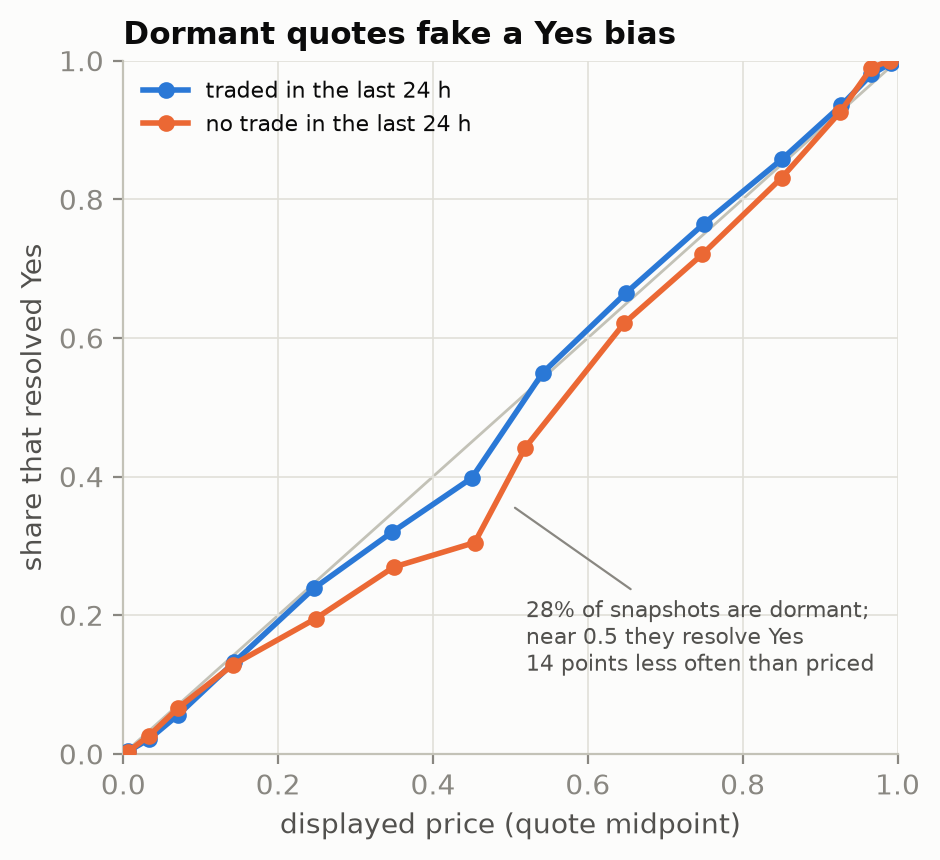
\includegraphics[width=0.37\linewidth]{../results/figures/midpoint_artifact.png}\hfill
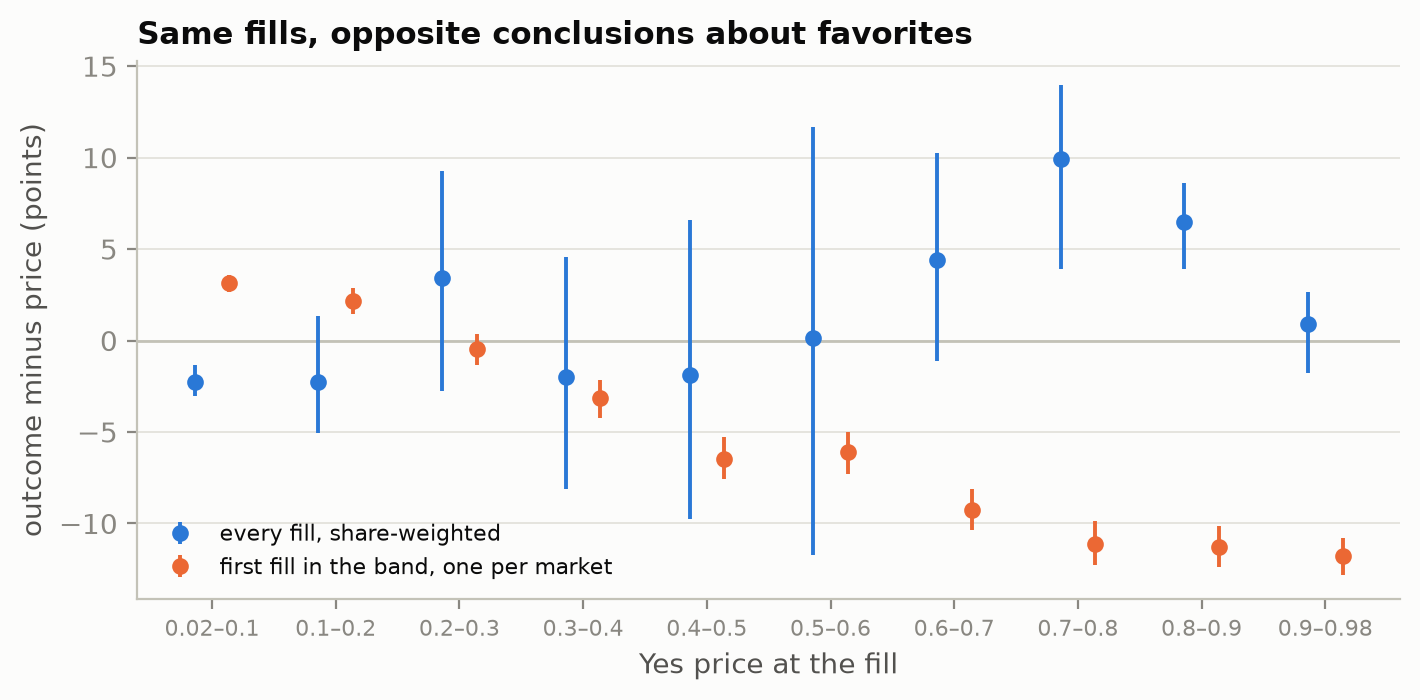
\includegraphics[width=0.61\linewidth]{../results/figures/estimators.png}
\caption{Left: reliability of displayed midpoints in long-tail Yes/No markets, split by whether the market traded in the prior day. Right: outcome minus price by Yes-price band on the same fills under two sampling rules. Whiskers are 95\% intervals from an event-level bootstrap.}
\label{fig:pitfalls}
\end{figure}

\subsection{What traded prices say}

At scheduled snapshots, last traded prices have a Brier score of \brierOverall{}. The logistic recalibration slope is below one in most categories (sports \slopeSports{}, politics \slopePolitics{}, weather \slopeWeather{}) and rises from \slopeEarly{} in the first 15\% of a market's life to \slopeLate{} in the last quarter. A slope below one means prices are slightly too extreme, the reverse of the compression reported from pooled trades, and consistent with last prints carrying transient noise early in a market's life.

Takers as a group earn \takerNet{} after fees: no measurable maker--taker transfer in aggregate, in contrast with Kalshi. The exception is crypto up/down contracts, where takers lose \updownTakerLoss{} and pay \updownFee{} of stake in fees.

\section{Event contracts as digital options}\label{sec:options}

A contract that pays one dollar if Bitcoin closes above $K$ at time $T$ is a cash-or-nothing call. With spot $S_t$, remaining time $\tau$, and volatility $\sigma$, a driftless lognormal model prices it at
\begin{equation}
\hat p_t=\Phi\!\left(\frac{\ln(S_t/K)-\tfrac12\sigma^2\tau}{\sigma\sqrt{\tau}}\right).
\end{equation}
Range contracts are differences of two such terms and one-touch contracts follow from the reflection principle. We set $\sigma$ to trailing realized volatility over a window of about four times the remaining horizon, use the last one-minute candle that closed before each fill, and fit nothing.

\begin{figure}[t]
\centering
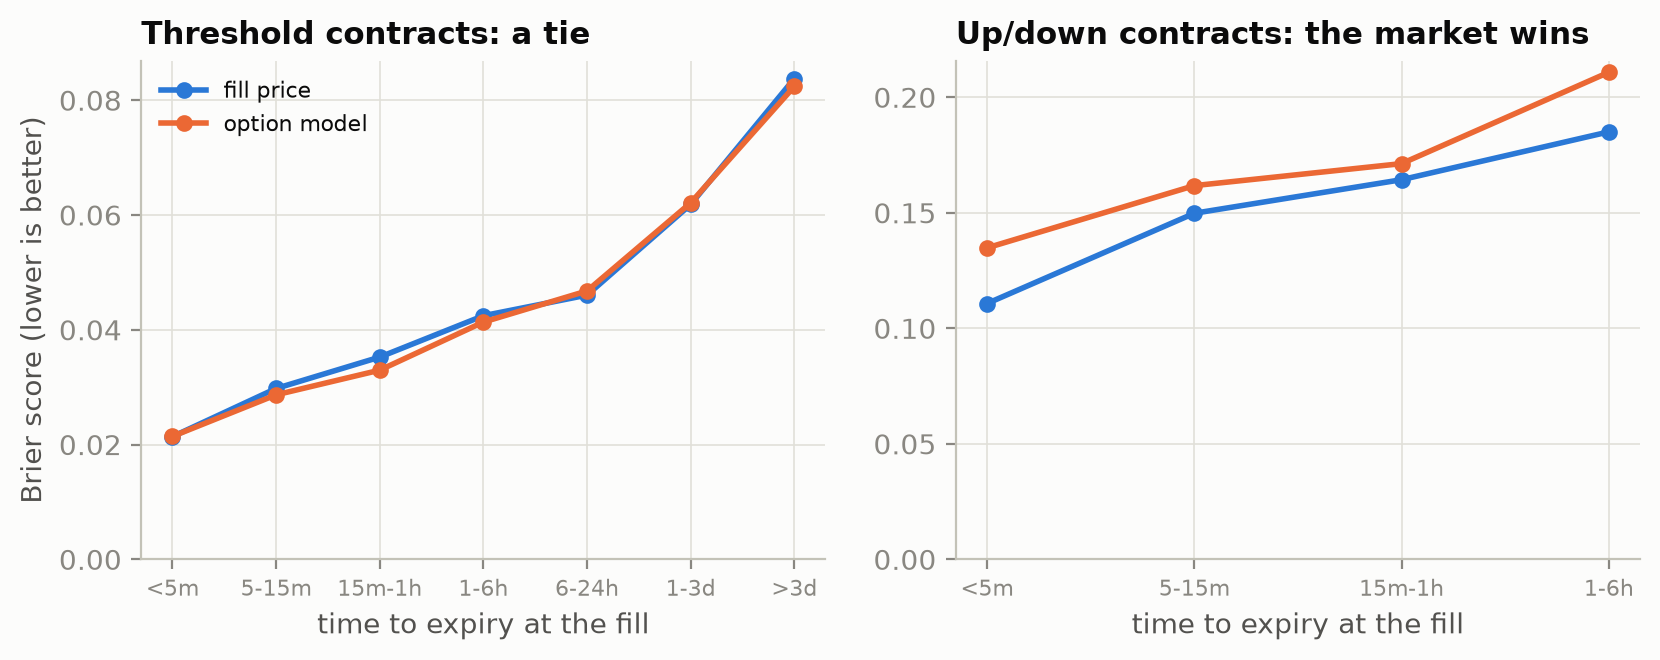
\includegraphics[width=0.56\linewidth]{../results/figures/options_brier.png}\hfill
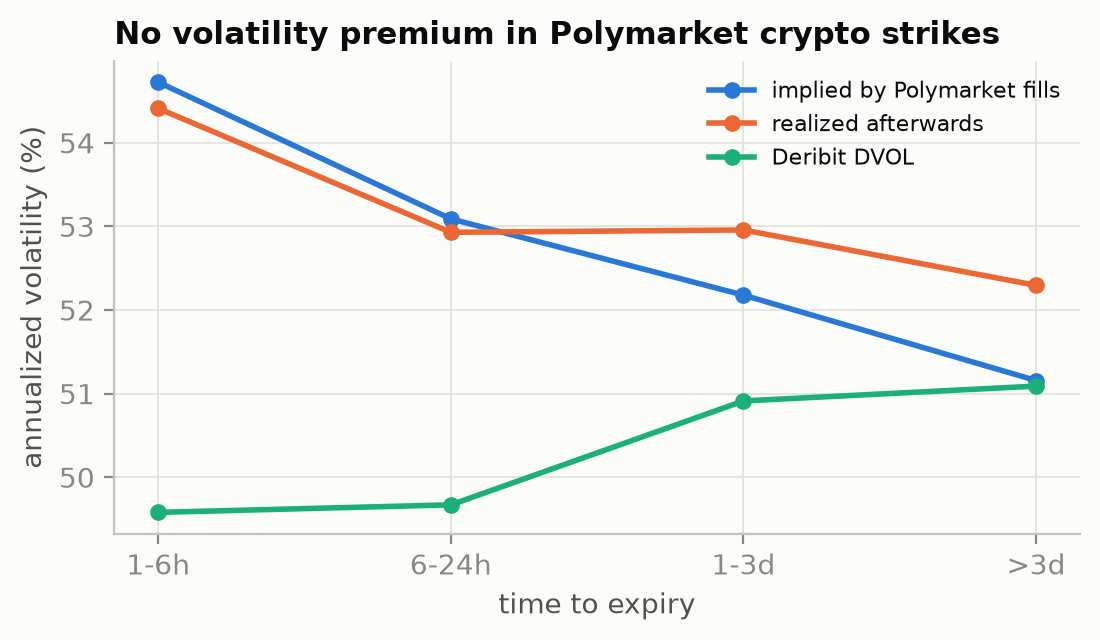
\includegraphics[width=0.40\linewidth]{../results/figures/implied_vol.png}
\caption{Left: Brier score of the fill price and of the option model at the same fills, by time to expiry. Right: volatility implied by Polymarket fills, volatility realized from the fill to expiry, and Deribit DVOL.}
\label{fig:options}
\end{figure}

\paragraph{Information.} Across \thrMarkets{} threshold contracts the model and the fill price are tied in Brier score at every horizon from five minutes to a week (Figure~\ref{fig:options}). In a logistic regression of the outcome on the log-odds of both, the price receives weight \encPrice{} and the model \encModel{}. The model is half of the best forecast. On short-dated up/down contracts the weight on the model is \encUpdown{}: that market already contains everything the formula knows.

\paragraph{No volatility premium.} Inverting the formula at each fill gives a Polymarket-implied volatility. Its ratio to the volatility realized between the fill and expiry lies between \ivRatioLow{} and \ivRatioHigh{} at every horizon. Listed options usually price volatility above what is realized; these contracts do not.

\paragraph{Fills the model endorses.} Call a taker fill endorsed when the model values the side the taker bought at least ten cents above the price paid plus the fee, and opposed in the mirror case. Endorsed fills in \backedMarkets{} markets (\$\backedStakeM{} million staked) returned \backedOne{} to the taker after fees, and opposed fills \opposedOne{}. When the model is given spot data that is 5, 15, and 60 minutes old, endorsed fills return \backedFive{}, \backedFifteen{}, and \backedSixty{} (Figure~\ref{fig:decay}). Most of the edge is a race to react to spot: at five and fifteen minutes the point estimates remain positive with intervals that reach zero, and at an hour nothing is left.

\paragraph{Single stocks.} The same construction on \stockMarkets{} contracts on the closes of large U.S. equities, with a trading-time variance clock and hourly bars, gives the model a weight of \stockEncModel{}. Takers who trade against it by ten cents lose \stockOpposedLoss{}, and still lose \stockOpposedStaleLoss{} when the model's bar is four hours older.

\begin{figure}[t]
\centering
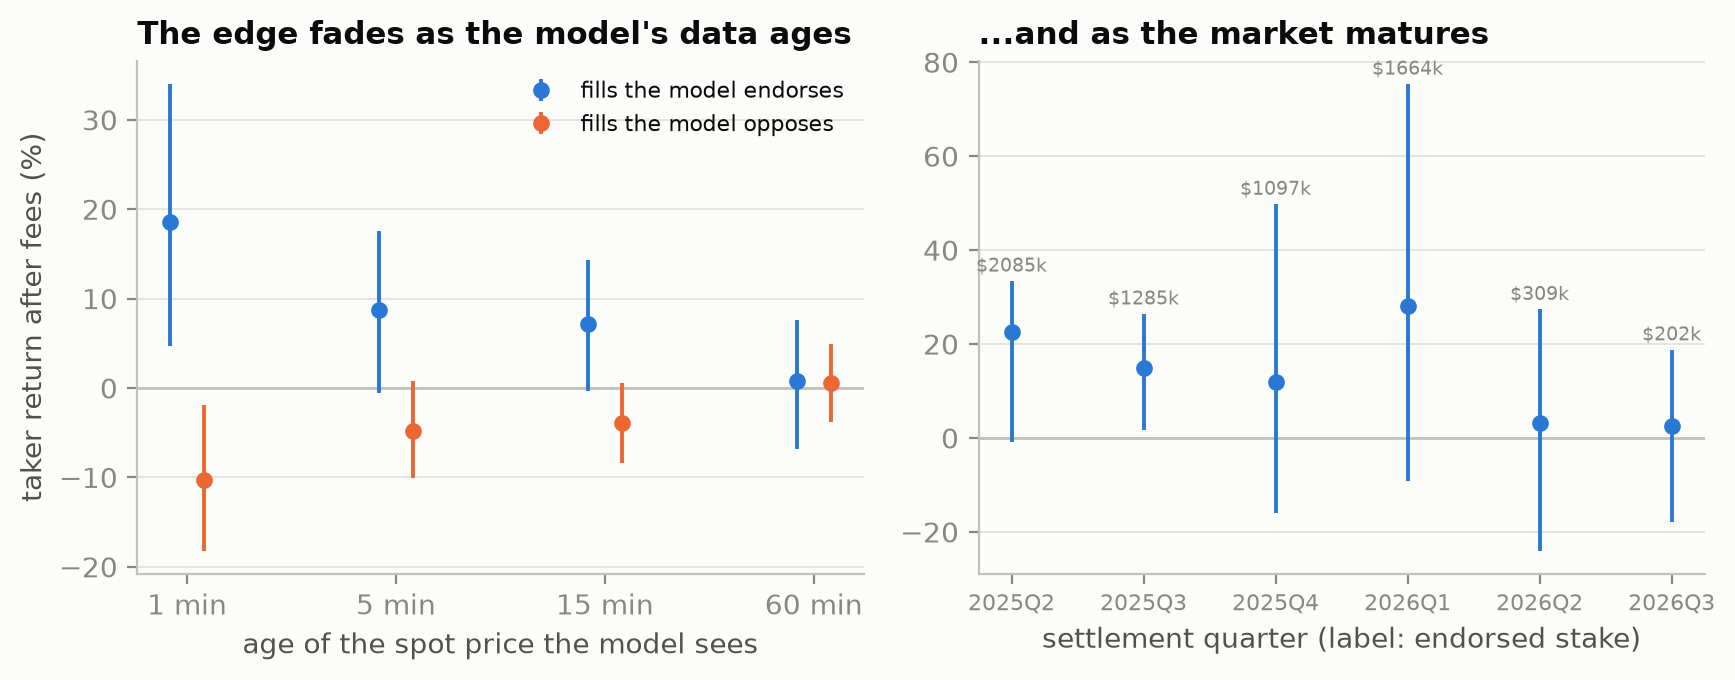
\includegraphics[width=0.66\linewidth]{../results/figures/edge_decay.png}
\caption{Taker return after fees on crypto threshold fills that the option model endorses or opposes by at least ten cents. Left: by age of the model's spot input. Right: endorsed fills by settlement quarter, with the stake they represent.}
\label{fig:decay}
\end{figure}

\section{Can anything else beat the price?}\label{sec:models}

\paragraph{Protocol.} Every challenger is evaluated walk-forward on the snapshot panel of Section~\ref{sec:data}. Test blocks are two calendar months. A model tested in a block is trained only on snapshots from markets that had resolved before the block began, so every training label was public when the test forecasts are made. The baseline is the last traded price. We report the change in Brier score relative to it with an event-level bootstrap over \modelTestMarkets{} test markets, and separately for the last five months (May to September 2026). No feature or setting was chosen on those months. They are not a pristine holdout: we saw scores for the same configurations on those months on an earlier tape half the size, and afterwards changed only the block length and the number of boosting rounds, to reduce compute.

\paragraph{Recalibration.} Platt scaling of the price changes the Brier score by \skillPlattAll{} overall and \skillPlattHold{} in the last five months (positive is better than the price); isotonic regression by \skillIsotonicAll{} and \skillIsotonicHold{}. Category-specific slopes do no better. The miscalibration these methods learn in one period is absent in the next. The quote midpoint, where a quote history exists, scores \skillMidAll{} relative to the last trade.

\paragraph{Learned residuals.} A gradient-boosted model of the residual $y-p$ returns the price itself when its features carry no signal. With price-path, order-flow, and wallet-record features its skill is \skillResFlowAll{} overall and \skillResFlowHold{} in the last five months. Adding the option-model value for price-linked contracts gives \skillResFullAll{} and \skillResFullHold{}. A two-parameter logistic blend of price and option value, which leaves all other contracts at the price, gives \skillBlendAll{} overall and \skillBlendHold{} in the last five months. On the \plMarkets{} price-linked test markets the blend improves on the last trade by \plSkillBlend{}, and on the quote midpoint at the same instant by \plMidBlend{} (change in Brier score \plMidBlendCI{}). Both feature families help out of time, and the option value contributes the larger share. By category the full model improves on the price in crypto thresholds, finance, culture, geopolitics, and mentions markets, is indistinguishable from it in sports, politics, economy, technology, and weather, and is worse on crypto up/down contracts. The pure formula, with nothing fitted, beats the displayed quote midpoint on price-linked contracts by \plMidFair{}: read as a forecast, the formula is better than the screen.

\begin{figure}[t]
\centering
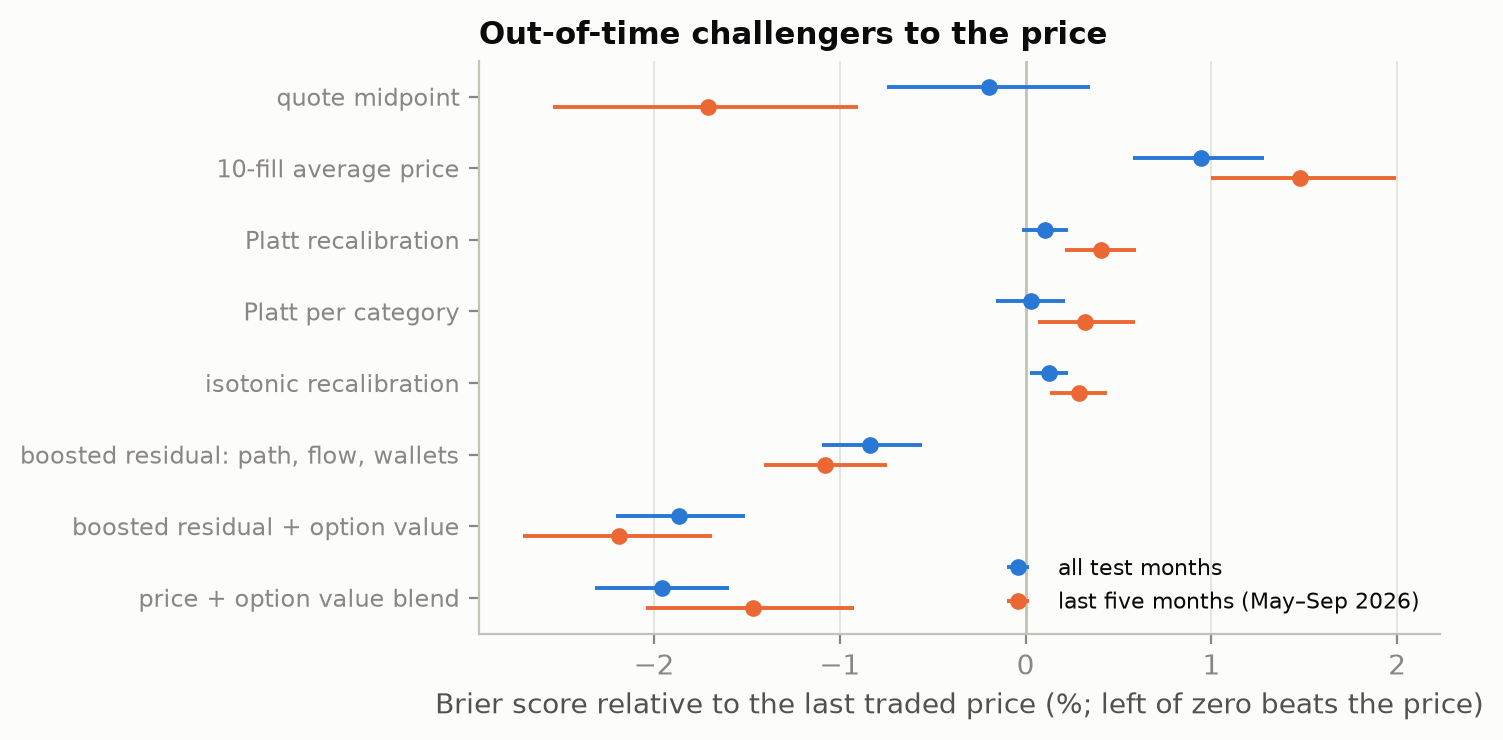
\includegraphics[width=0.56\linewidth]{../results/figures/models.png}\hfill
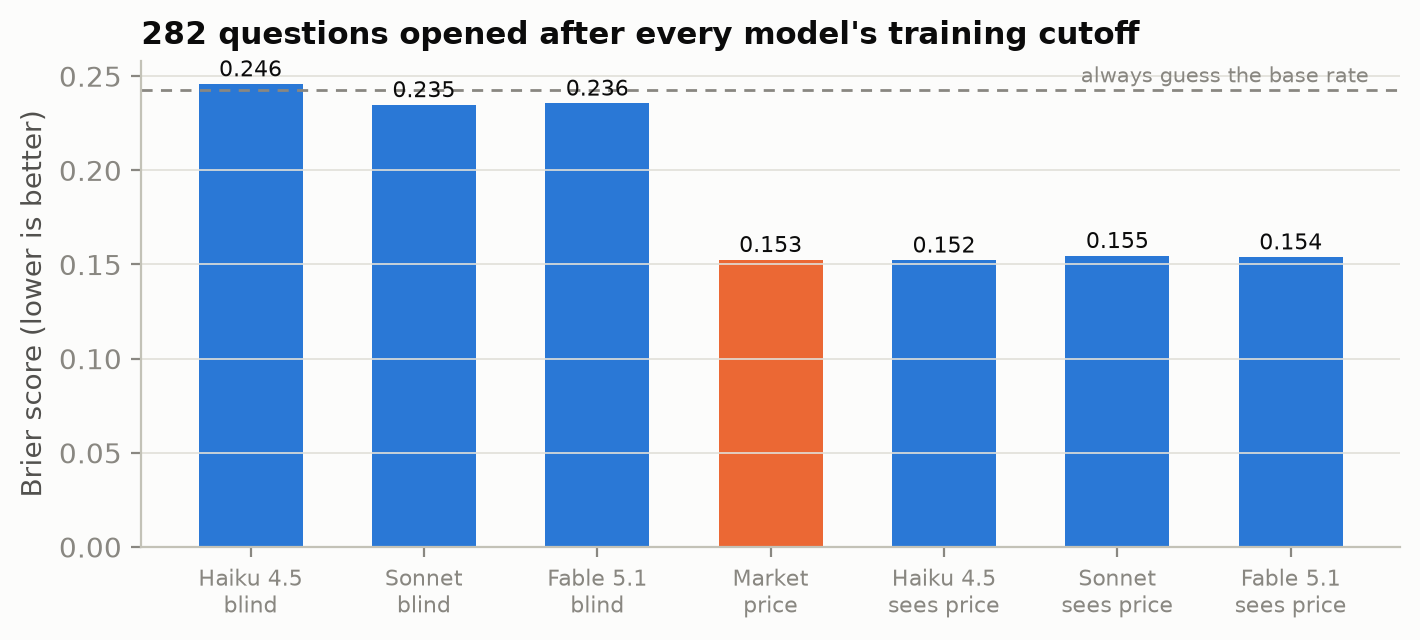
\includegraphics[width=0.42\linewidth]{../results/figures/llm.png}
\caption{Left: Brier score of each challenger relative to the last traded price, walk-forward, with 95\% event-bootstrap intervals. Right: language-model forecasts on questions opened after the models' training cutoffs, with and without the market price in the prompt.}
\label{fig:models}
\end{figure}

\paragraph{Wallet records.} For each fill we compute the taker wallet's realized return on markets that had resolved before the fill. Fills by wallets with no resolved history return \firstTimers{} after fees and fills by seasoned wallets \seasoned{}. Within seasoned wallets, sorting by past return does not sort future return. Our tape covers a sample of markets, so each wallet's record is partial, and this null is weaker evidence than the full-chain result of \citet{gomezcram2026prediction}.

\paragraph{Language models.} We select \llmN{} Yes/No markets that opened after 10 July 2026, one per event, across ten categories, and fix a forecast date at 30\% of each market's scheduled life. Three Claude models (Fable 5.1, Sonnet, Haiku 4.5) receive the question, the resolution rules, and the date, with no tools and no retrieval; each run was verified to have made only the file read and write that the protocol requires. Blind, they score \llmBlindFable{}, \llmBlindSonnet{}, and \llmBlindHaiku{} against a market Brier score of \llmMarket{} and \llmBase{} for a constant base-rate forecast. Shown the market price, they score \llmPriceFable{}, \llmPriceSonnet{}, and \llmPriceHaiku{}, and the weight on the model in a regression that includes the price is not distinguishable from zero. Without news access a language model knows the base rate and nothing the market does not.


\section{What survives}\label{sec:survives}

\paragraph{A capital-constrained replay.} We replay the option-model rule on crypto threshold fills with a \$200 cap per fill, the model's spot input fifteen minutes old, and profit booked at expiry. The threshold of ten cents was chosen using contracts that expired before April 2026; later contracts form a confirmation period. Over the whole sample the rule returns \replayAll{} on stake with at most \$\replayCapitalK{} thousand deployed, an annualized Sharpe ratio of \replaySharpe{} ($t=\replayT$ on daily returns), and a deflated Sharpe probability of \replayDSR{} after discounting for the 24 variants we examined. The pooled fill-level interval excludes zero; the daily series does not. In the confirmation period it returns \replayConfirm{} ($t=\replayConfirmT$). By \lastQuarter{}, endorsed fills return \lastQuarterEndorsed{}. Two things changed: a seven-percent taker fee rate reached every crypto contract in the second quarter of 2026, and the stake that clears a ten-cent bar fell by an order of magnitude. The single-stock rule is smaller and cleaner: \stockReplayAll{} on stake with at most \$\stockReplayCapitalK{} thousand deployed, a Sharpe ratio of \stockReplaySharpe{}, a deflated Sharpe probability of \stockReplayDSR{}, \stockReplaySelect{} before April 2026 and \stockReplayConfirm{} after.

\begin{figure}[t]
\centering
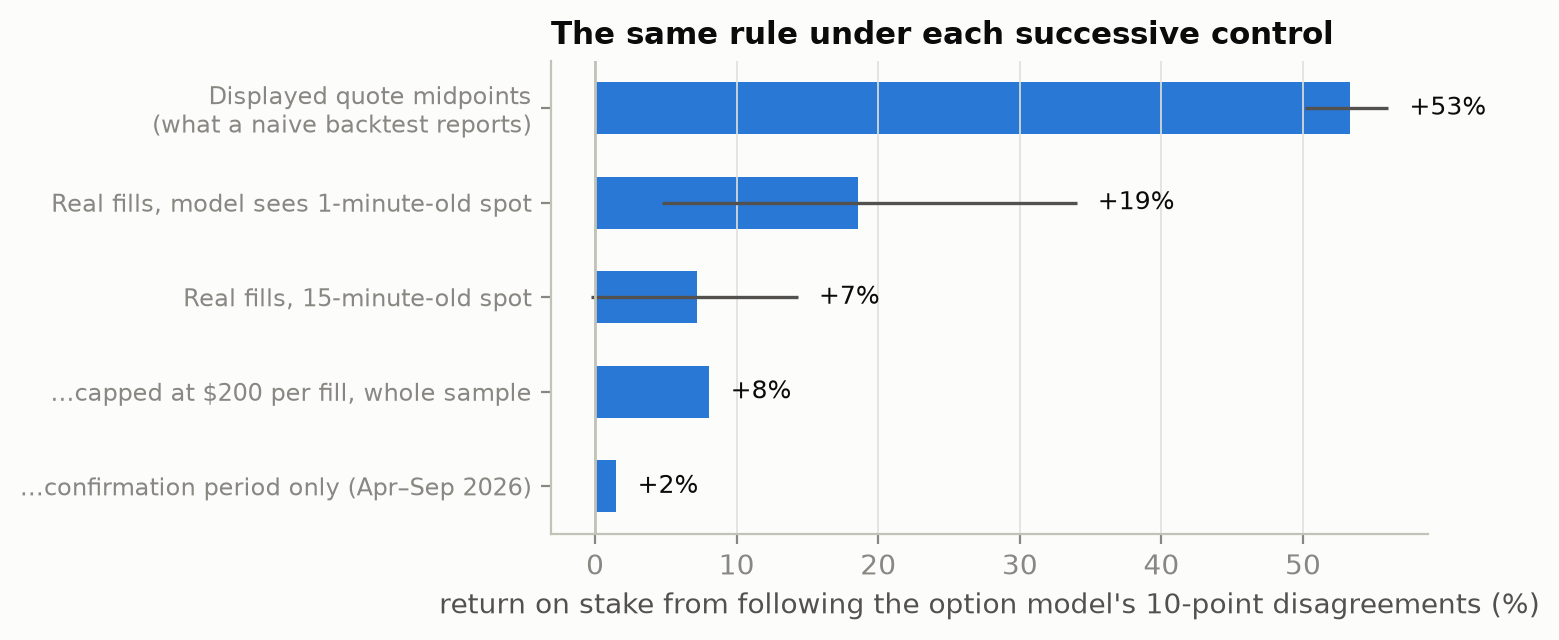
\includegraphics[width=0.60\linewidth]{../results/figures/ladder.png}
\caption{Return of one rule, ``follow the option model when it disagrees with the price by ten cents,'' under successive controls.}
\label{fig:ladder}
\end{figure}

\paragraph{First touch.} The overshoot of Section~\ref{sec:pitfalls} can be traded only at prices that exist later. After the first fill of a market inside a Yes-price band, we buy No at the next fill in which a taker bought No at least 60 seconds later, provided the Yes price is still within five cents of the band. The median wait is \fadeWait{} minutes. Net of fees the fade returns \fadeMid{} on stake for the band 0.6 to 0.8 (\fadeMidN{} markets) and \fadeHigh{} for 0.8 to 0.98 (\fadeHighN{} markets). From April 2026 onward the returns are \fadeMidLate{} and \fadeHighLate{}. Dropping the trigger and taking each market's first No-buying fill in the same price range returns \fadeMidBase{} and \fadeHighBase{}, so the result does not depend on reacting to the first print. Its limit is size: the fills copied have a median stake of \$\fadeFillUsd{} and total \$\fadeTotalK{} thousand across both bands. Where the move into the band is sustained over the next five fills, the level it settles at still exceeds the outcome frequency by \sustainedGapMag{} points.

\section{Discussion}

\paragraph{For an investor.} Four things carry over to any market where a price is read as a probability. First, a displayed price is evidence only if someone could trade there; dormant quotes created the largest bias in our data. Second, the sign of a bias can depend on the sampling rule, so an estimate should come with a rule that could be executed. Third, a contract with a traded underlying can be priced from the underlying, and where that price disagrees with the market by a wide margin the market was the one that was wrong, although the disagreement has become rarer and fees have absorbed most of it. Fourth, the amounts are small: the option-model rule never deployed more than a few hundred thousand dollars.

\paragraph{Limitations.} Fills are a stratified sample, so wallet histories are partial and wallet-level conclusions are weak. The trade feed reports the taker side only. Spot inputs for stock contracts are hourly and blind to extended-hours trading. We observe fills, not order books, so the capacity of each rule is bounded above by the sizes that traded. Chainlink-settled contracts are modeled with Binance prices. The confirmation period is six months. Literature values quoted in Section~2 are as reported by their authors.

\paragraph{Conclusion.} Most measured mispricing on the largest prediction market is produced by how it is measured. What remains is concentrated where a public model of the underlying exists and where thin books let a single order move the price, and both remainders are shrinking.

\bibliographystyle{ACM-Reference-Format}
\bibliography{refs}

\end{document}
